\section{iClusterVB Implementation on simulation data}

In this section, we show how the \textbf{iClusterVB} method works using simulated  data. 
The data includes 240 individuals and 4 different types of data views. 
These data types are often found in genomics studies:

\begin{itemize}
  \item Two continuous views (like gene expression)
  \item One binary view (like mutation: yes or no)
  \item One count view (like DNA copy number)
\end{itemize}

Each view has 500 features, so in total we have 2000 features. But only 10\% of features (50 per view) are useful for clustering. The rest are just noise (not important).

The true number of clusters is 4, and each cluster has the same number of individuals (60 each).
\\

We combined these datasets into a list and specified their types using a vector. Before running the model, we changed the 0 values in the binary data to 2, because the algorithm does not accept zeros. 
Then, we used the iClusterVB function to run the clustering model with a maximum of 8 clusters.
The model correctly found 4 clusters. After that, we used summary to check the results and piplot and 
chmap to visualize selected features and clusters. 

\begin{table}[!h]
  \centering
  \caption{Summary of Clustering and Variable Selection Results}
  \label{tab:clustering_summary}
  \begin{tabular}{llc}
  \toprule
  \textbf{Category} & \textbf{Description} & \textbf{Value} \\
  \midrule
  \multicolumn{3}{c}{\textit{Clustering Hyper-Parameters/Result}} \\
  \midrule
  Number of individuals & Total number of observations & 240 \\
  Maximum clusters specified & User-defined input & 6 \\
  Number of clusters found & Determined by algorithm & 4 \\
  Individuals per cluster & Cluster sizes (equal) & 60 \\
  \midrule
  \multicolumn{3}{c}{\textit{Variable Selection by View (Threshold: 0.5)}} \\
  \midrule
  View 1 (Gaussian) & Variables selected & 57 out of 500 \\
  View 2 (Gaussian) & Variables selected & 58 out of 500 \\
  View 3 (Multinomial) & Variables selected & 63 out of 500 \\
  View 4 (Poisson) & Variables selected & 68 out of 500 \\
  \bottomrule
\end{tabular}
\end{table}

The clustering algorithm identified a total of 4 clusters from the simulated dataset,
 despite a user-specified maximum of 6 clusters. Each cluster contains exactly 60 individuals,
  summing to a total of 240 individuals.

Variable selection results indicate the number of variables exceeding a posterior inclusion
probability threshold of 0.5 in each view. Specifically, 57 and 58 variables were selected in
View 1 and View 2, respectively (both Gaussian views), while 63 variables were selected in View 3
(Multinomial view), and 68 variables in View 4 (Poisson view), out of a total of 500 variables per view.
These results suggest meaningful contributions from all data types, with slightly stronger signals
from the Multinomial and Poisson views.

\begin{table}[!h]
  \centering
  \caption{Cross-tabulation of Predicted vs. True Cluster Memberships}
  \label{tab:confusion_matrix}
  \begin{tabular}{ccccc}
  \toprule
  \textbf{Predicted Cluster} & \textbf{True Cluster 1} & \textbf{True Cluster 2} & \textbf{True Cluster 3} & \textbf{True Cluster 4} \\
  \midrule
  1 & 0 & 0 & 60 & 0 \\
  2 & 0 & 60 & 0 & 0 \\
  3 & 60 & 0 & 0 & 0 \\
  6 & 0 & 0 & 0 & 60 \\
  \bottomrule
\end{tabular}
\end{table}

Table~\ref{tab:confusion_matrix} presents the cross-tabulation between the predicted cluster 
labels and the true underlying cluster assignments. Each predicted cluster perfectly matches 
one of the true clusters without any misclassification. Specifically, predicted cluster 1 matches
 true cluster 3, cluster 2 matches true cluster 2, cluster 3 matches true cluster 1, and cluster 
 6 corresponds exactly to true cluster 4. This result indicates a perfect clustering performance, 
with all 240 individuals correctly assigned to their respective groups.

\begin{figure}[!h]
  \centering
  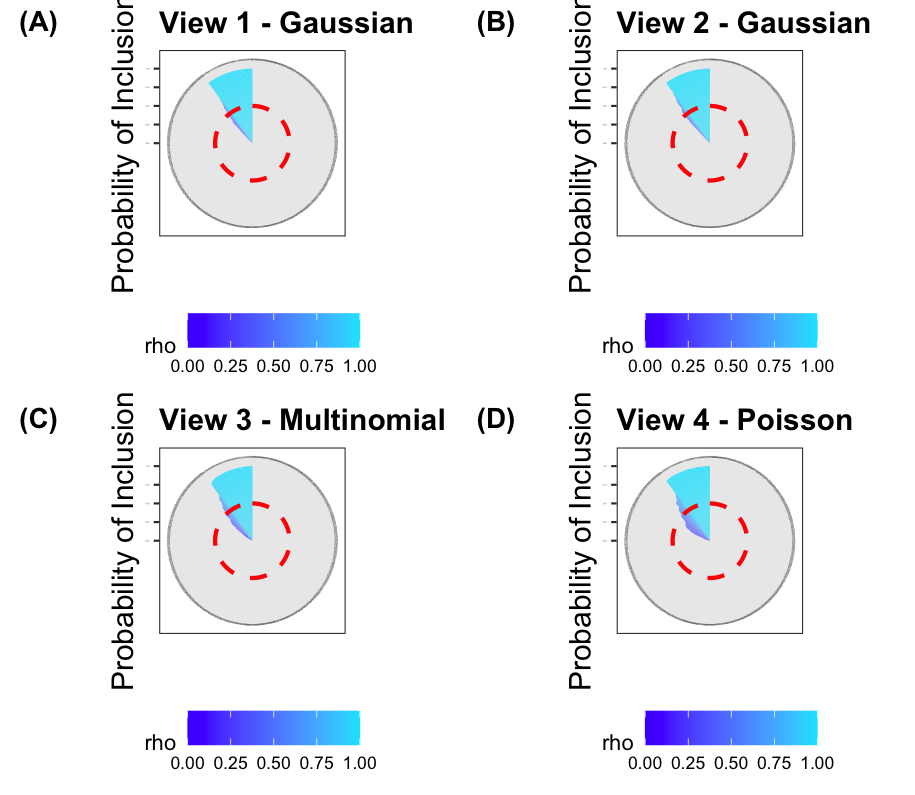
\includegraphics[width=0.7\textwidth]{../results/piplot_sim_data.png}
  \caption{PIP plot showing the posterior inclusion probabilities (PIPs) of features across all data views.}
  \label{fig:piplot}
\end{figure}

Figure~\ref{fig:piplot} illustrates the posterior probability of variable inclusion across
 the four different data views: (A) and (B) correspond to the two Gaussian views, 
 (C) corresponds to the Multinomial view, and (D) to the Poisson view.
  In each subplot, the radial axis represents the probability of inclusion for individual variables,
   with higher values indicating stronger evidence of variable relevance.
    The angular separation reflects the clustering structure among variables.

The color gradient encodes the \(\rho\) value, which governs the correlation or dependence strength across features. Bright blue regions (high \(\rho\)) indicate confidently selected variables, while darker tones indicate low inclusion probability or noise. Across all views, the most informative variables are highlighted clearly with high inclusion probabilities concentrated in narrow angular bands, consistent with the true signal structure of the simulated dataset.


\begin{figure}[!h]
  \centering
  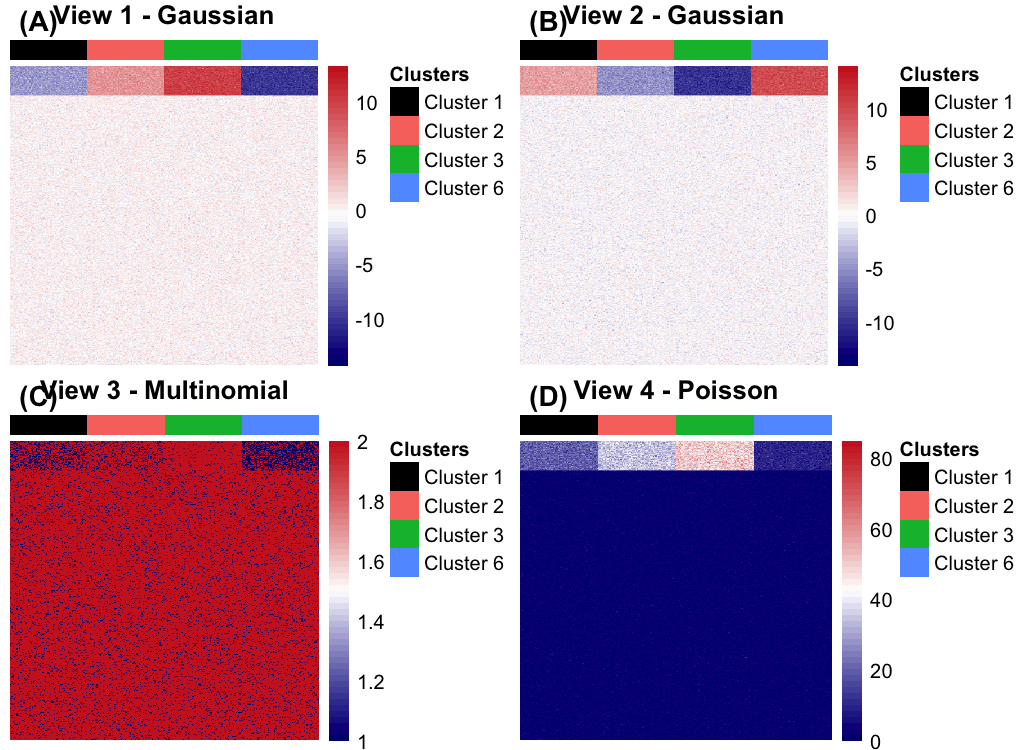
\includegraphics[width=0.7\textwidth]{../results/hamp_sim_data.png}
  \caption{Cluster heatmap showing the clustering structure and variable selection across all data views.}
  \label{fig:chmap_sim_data}
\end{figure}

Figure~\ref{fig:chmap_sim_data} shows heatmaps of the four data views used for clustering. 
Clear block patterns in Views 1 and 2 (Gaussian) indicate that these features distinguish clusters well. 
View 3 (Multinomial) also displays cluster-specific structure in the upper rows. 
While View 4 (Poisson) is mostly sparse, the top block shows variation across clusters, suggesting some informative features. 
Together, these heatmaps validate that each view contributes to identifying distinct clusters.

% ----------------above are moved to vscode for refining--------